%tabulacao para a listagem
%\newcommand{\itab}[1]{\hspace{0em}\rlap{#1}}
%\newcommand{\tab}[1]{\hspace{.2\textwidth}\rlap{#1}}

%inicio do capitulo
\chapter[INTRODUÇÃO]{INTRODUÇÃO}

A capacidade e necessidade de se comunicar surge desde o berço, fruto de educação, podendo ser expressada de várias formas, seja ela escrita ou  oral \cite{falcao2014leitura}. A comunicação é a vantagem evolutiva humana quando comparado com os demais seres que existem, pois através dela é possível trocar informações uns com os outros, possibilitando a elaboração de ideias para sobreviver e enfim dominar o mundo ao seu redor \cite{dos2018importancia}.  

Para permitir que a máquina consiga compreender e reproduzir as formas de comunicação humana, cientistas e engenheiros estudam uma área de
pesquisa de Processamento de Linguagem Natural (NLP, do inglês \textit{Natural language processing}), que envolve várias aplicações, tais como:
\begin{itemize}
    \item Sumarização automática: produz um resumo legível de uma parte do texto. 
    \item Reconhecimento de locutor: identificação da pessoa através da voz \cite{campbell1997speaker}, podendo ser utilizado como mecanismo de segurança em alguns sistemas.
    \item Análise de subjetividade (\textit{sentiment analysis} ou \textit{opinion mining}): Extrai informações subjetivas geralmente de um conjunto de documentos, muitas vezes usando revisões online para determinar a ``polaridade'' sobre objetos específicos. É especialmente útil para identificar tendências da opinião pública nas mídias sociais, para fins de marketing \cite{ding2014sibgrapi}.
    \item Desambiguação: muitas palavras têm mais de um significado, assim temos que selecionar o significado que faz mais sentido no contexto.
    \item Extração de relacionamento: identifica as relações entre entidades nomeadas (por exemplo, quem é casado com quem) com base em textos.
    \item Segmentação morfológica: separa palavras em morfemas individuais e identifica classes de morfemas.
\end{itemize}

Este trabalho versa sobre a aplicação denominada de  Reconhecimento Automático de Fala (ASR, do inglês \textit{Automatic Speech Recognition}) ou também conhecido por sistemas \textit{Speech-To-Text} (literalmente, Fala-para-Texto). O ASR  consiste no processo de conversão de um sinal acústico em um conjunto de palavras que foram ditas  \cite{voiceinteraction}. O primeiro sistema de reconhecimento de fala conhecido e documentado foi construído em 1952 por Davis, Biddulph e Balashek em Bell Laboratories, sistema era capaz de reconhecer dígitos, alcançando precisão de 97-99\% quando era adaptado ao falante \cite{juang2005automatic} \cite{pieraccini2012audrey}. Posteriormente, surgiram diversos usos para o reconhecimento de fala, como ferramenta de interação entre humano e máquina, por exemplo:

    \begin{itemize}
        \item Aplicativos, como Siri, Cortana e Google Assistant, que permitem que o usuário acione funções ou realize buscas através de comandos de voz \cite{lopez2017alexa};
        \item Atendimento ao cliente via de \textit{chatbots} \cite{raju2018contextual}.
        \item Tecnologias Assistivas, como por exemplo em \citeonline{lima2015reconhecimento}, em que é desenvolvido um ambiente virtual para pessoas cegas.
        \item Legendas automáticas de vídeos.
        \end{itemize}


A \autoref{fig:fluxo} ilustra o fluxo do ASR, que se inicia com o usuário falando uma frase ao sistema \cite{cpqd}. A frase corresponde a um sinal de áudio, marcado por um retângulo verde. O sinal de áudio é processado pelo motor de reconhecimento de fala, que converte o áudio para texto. 

\begin{figure}[h!]
\centering
\caption{Fluxo geral do reconhecimento.}
\label{fig:fluxo}
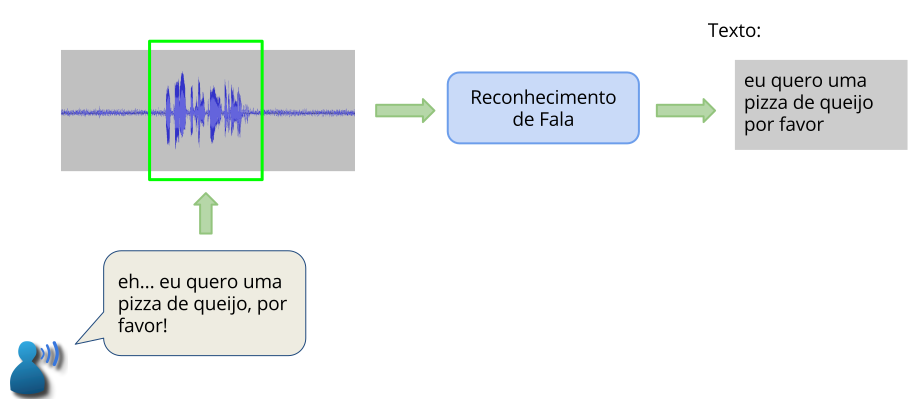
\includegraphics[width=\textwidth]{images/asr-flow.png}
\fonte{\citeonline{cpqd}.}
\end{figure}


%\todo[inline]{DEFINIÇÃO DE TRANSCRIÇÃO, vantagens e aplicações}

%As principais vantagens para o seu uso é a facilidade de registrar informações, realizando o processo de forma automática e muito mais rápida quando comparado com o trabalho manual. Também deve ser notado o benefício de alterar o formato de um vídeo para texto para impulsionar a divulgação, fazendo com que alcance mais pessoas que preferem ler um texto. De forma ainda mais específica na questão "alcançar mais pessoas", é de grande importância na acessibilidade de deficientes auditivos que não conseguiriam compreender o conteúdo do áudio \cite{litero}.

A transcrição da fala pode facilitar e trazer conforto ao dia a dia permitindo abrir aplicativos e digitar textos através da fala  \cite{litero}. Porém seu uso não se limita a isso, atualmente também é utilizado em ambientes corporativos, elevando muito a produtividade de tarefas. Por exemplo, empresas que realizam muitas reuniões, transcrevendo as atas diretamente de áudio para texto, aumentando a produtividade ao automatizar essas tarefas. No campo judiciário também possui grande destaque, uma vez que podem substituir o digitador responsável por documentar toda a sessão em formato de texto, otimizando o tempo e recursos que podem ser alocados para outras tarefas. Além disso, vale ressaltar também o uso em: investigações, escutas telefônicas, gravação de depoimentos, audiências, sessões parlamentares, transcrição de aulas, adaptação de conteúdos para deficientes auditivos,  dentre outros \cite{computerworld}. 

%\section{DIFICULDADES}

%\todo[inline]{dissertação do braccent tem muita informação e referencia interessante}
No exemplo apresentado na \autoref{fig:fluxo}, nota-se que a frase resultante do sistema não é exatamente a mesma, a parte inicial ``eh...'', que indica uma certa hesitação da pessoa não foi convertida, bem como os símbolos de pontuação ',' e '!' também não foram compreendidas pelo sistema. A exclamação tem a ver com entonação da voz da pessoa, e pontuações em geral, ainda é um tema em estudo \cite{zelasko2018punctuation}. Outro tema em estudo é o cenário em que há várias pessoas conversando simultaneamente \cite{sudoh2020simultaneous}. Um fator que pode dificultar o ASR é a qualidade do áudio e o ruído ambiente que podem confundir o sistema \cite{sharan2016overview}. 

\begin{figure}[h!]
\centering
\caption{Mapa de dialetos do português brasileiro}
\label{fig:mapa}
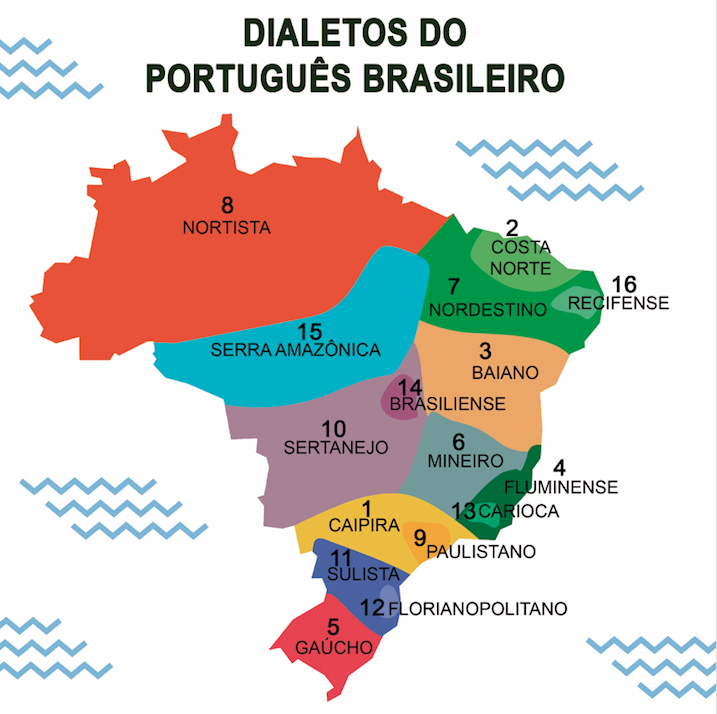
\includegraphics[width=0.5\textwidth]{images/dialeto-portugues.png}
\fonte{\citeonline{dialetoportugues}.}
\end{figure}

Também devemos levar em consideração a língua falada, pois dependendo da língua, os recursos disponíveis variam. A língua inglesa é a que possui mais estudos e por consequência uma maior base de dados, modelos e resultados para trabalhar comparado à língua portuguesa, por exemplo. Outra  questão é que há diferentes sotaques para a mesma língua dependendo da região, como é possível observar no mapa da \autoref{fig:mapa}, que apresenta uma divisão do território brasileiro por sotaque. Cada sotaque pode ter uma diferente pronúncia para algumas palavras, o que pode confundir o sistema de reconhecimento de fala \cite{viglino2019end}. 
%Por esses motivos o reconhecimento de fala processando a língua portuguesa acaba obtendo uma menor taxa de acertabilidade quando comparado ao inglês \cite{alvarenga2019transcriccao}.

 %\cite{waibel1990readings}
 %e o tamanho do vocabulário pode aumentar a complexidade caso seja muito grande.
%não possui em domínio público um sistema de reconhecimento automático de voz para o português, com suporte a grandes vocabulários. 

\section{A PROPOSTA}


A proposta deste trabalho é comparar Applications Programming Interface (API),  que tem o serviço de ASR para a língua portuguesa, em uma base de dados com sotaques regionais brasileiros distintos. 
Ha várias APIs no mercado, a página \citeonline{listaAPI} contém uma lista das 10 que o autor considera as melhores do mercado. As APIs foram selecionadas levando em consideração se são renomadas ou não e quais processam a língua portuguesa (pt-BR). 
Outra quesito que foi considerada é o custo de sua utilização. A fim de reduzir o custo do desenvolvimento do trabalho, todas as APIs devem ser gratuitas ou disponibilizem de forma gratuita por um quantidade pré-definida de período/uso. Ao final, foram selecionadas duas APIs: Google Cloud Speech API\footnote{https://cloud.google.com/speech-to-text} e Wit.ai\footnote{https://wit.ai/}. 
%Já sabemos que para o inglês apresenta ótimos resultados, uma vez que as primeiras aplicações foram feitas baseadas na língua, o que justifica um maior desenvolvimento para ela.

Como fonte de dados foi utilizado a base de dados Braccent, criada por \citeonline{batista2019estudo}, que é uma base de áudios com grande diversidade de sotaques. Foi usado um subconjunto de 1.648 áudios da base de dados Braccent. As gravações são identificadas de acordo com o gênero e o sotaque regional falado na locução, sendo 854 amostras do sexo feminino e 794 amostras do sexo masculino. Os sotaques são: nortista, baiano, fluminense, mineiro, carioca, nordestino e sulista. Além da informação do sotaque, há ainda a informação de grau de escolaridade: médio incompleto, médio completo, superior incompleto, superior completo, mestrado e doutorado. Assim, será possível comparar os resultados por fatores regionais, culturais e naturais  \cite{correiacomunicaccao}: 

\begin{itemize}
    \item Fatores regionais: é a diferença do português falado por uma pessoa nascida e criada na região nordeste e outro na região sul do Brasil. 
    \item Fatores culturais: o grau de escolarização e a formação cultural de uma pessoa são fatores que podem soar diferentemente aos ouvidos de outra pessoa. 
    \item Fatores naturais: o uso da língua pelos falantes sofre influência de fatores naturais, como idade e sexo. Uma criança não fala da mesma forma que um adulto.
\end{itemize}


A escolha dessa base foi feita justamente para analisar o comportamento destas APIs quando utilizadas para processar toda a variedade do pt-BR. A \autoref{diagramaAPIintro} apresenta a arquitetura geral do ambiente de testes desenvolvido usando a linguagem de programação Python que usará as duas API para transcrição dos áudios da base de dados Braccent. Para analisar a taxa de acerto da transcrição da fala foram utilizadas as métricas Levenshtein e  Levenshtein Normalizado. 

\begin{figure}[h!]
\centering
\caption{Modelo de funcionamento.\label{diagramaAPIintro}}
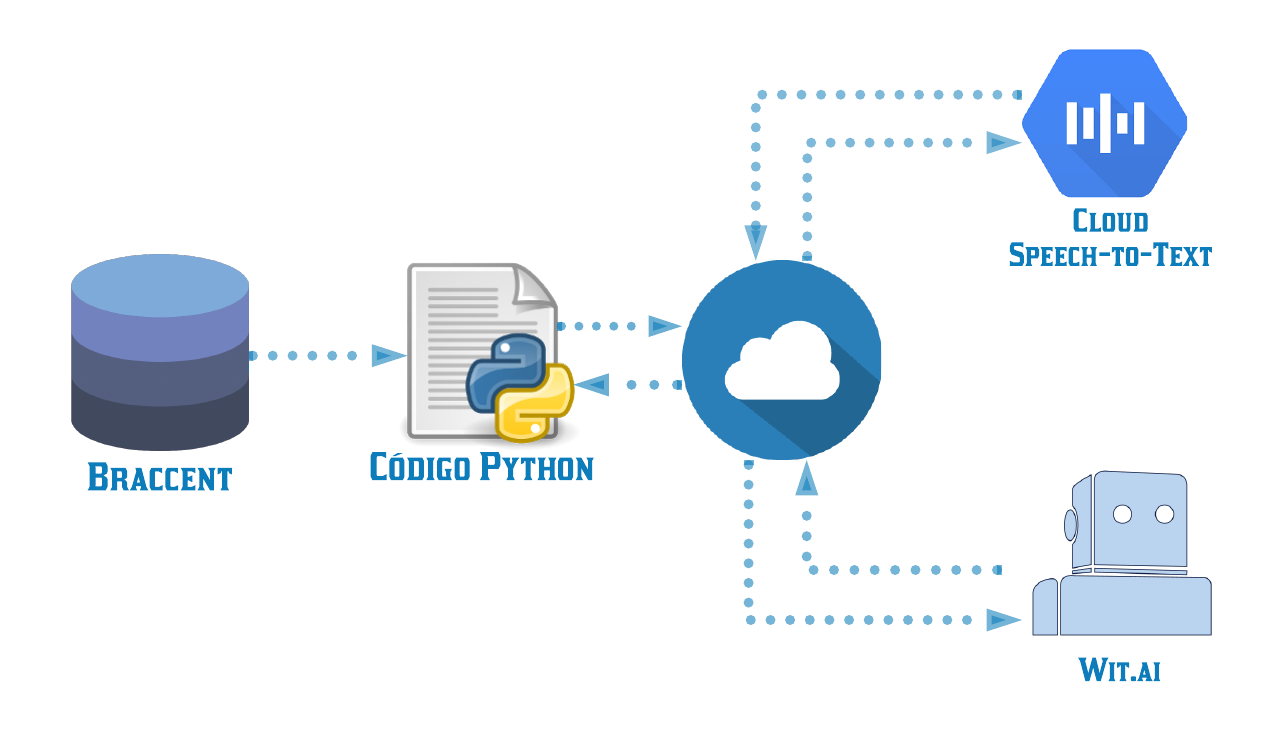
\includegraphics[width=115mm]{images/Diagramas/APIs.png}
\fonte{elaborado pelo próprio autor (2021)}
\end{figure}


%\todo[inline]{Terminar de escrever a parte de métricas de erro após a finalização do cap4}
%para analisar a taxa de acerto da transcrição da fala através da métrica WER, coletando os áudios para teste da base de dados Braccent.
%No processo de transcrição algumas palavras podem ser transcritas de forma errada, para calcular taxa de erros de uma transcrição, 

%uma métrica utilizada para mensurar a precisão de aplicações de ASR denominada Word Error Rate (WER), sendo basicamente a soma do número de palavras substituídas, inseridas e deletadas dividido pelo número de palavras totais \cite{wer}.

%\begin{itemize}
    %\item palavras substituídas: uma palavra é substituída por outra, por exemplo: trocar comprimento por cumprimento;
    %\item palavras inseridas: uma palavra que não foi dita é incluída no texto transcrito, por exemplo:
    %\item palavras deletadas: uma palavra que foi dita porém não foi incluída no texto transcrito, por exemplo: "jogue isso assim" vire "jogue assim".
%\end{itemize}


\section{OBJETIVOS}
\subsection{Objetivo Geral}

O objetivo deste trabalho é comparar a taxa de acerto da transcrição da fala em língua portuguesa, levando em consideração diferentes sotaques regionais brasileiros, graus de escolaridade e gêneros, das ferramentas Google Cloud e Wit.ai.

\subsection{Objetivos Específicos}

Os objetivos específicos identificados para se atingir o objetivo geral proposto são:
\begin{itemize}
    \item Pesquisar sobre as APIs, Google Speech API e  Wit.ai.
    \item Pesquisar sobre as métricas de comparação de \textit{strings}.
    \item Desenvolver ambiente dos experimentos, com coleta de dados e estatísticas.
\end{itemize}


%\section{LIMITAÇÕES}

\section{ESTRUTURA DO TEXTO}

Este trabalho está dividido em cinco capítulos. Este primeiro capítulo trouxe uma introdução ao problema estudado, a contextualização do tema, a justificativa para a sua realização e os objetivos pretendidos.  O Capítulo 2 apresenta detalhes da base de dados Braccent e das ferramentas Google Speech API e  Wit.ai, além do detalhamento da métrica de Levenshtein. Em seguida, o Capítulo 3 traz o desenvolvimento do sistema e o Capítulo 4 traz os resultados dos áudios processados e a discussão associada. Por fim, no Capítulo 5, são tecidas as considerações finais e os trabalhos futuros.

\begin{comment}
Por conta da tecnologia existente na época, os resultados não eram tão significativos, o que fazia com que o Reconhecimento de Fala não tivesse tanta visibilidade. Porém por causa de diversos motivos ligados ao avanço tecnológico da humanidade estamos tendo cada vez mais contato com ASR. \citeonline{yu2016automatic} citam 3 fatores para estarem ocorrendo essas mudanças, elas são:

\begin{itemize}
    \item O poder computacional que está disponível;
    \item O avanço da internet contribuindo com a quantidade de acesso a mais dados;
    \item O uso cada vez maior de dispositivos portáteis (\textit{smartphones}, \textit{smartwatches}, dentre outros).
\end{itemize}

   
%Todos esses vários usos  do Reconhecimento de Fala possuem obstáculos em comum que dificultam a sua implementação. 

%Comumente estamos habituados a falar conectando as palavras uma nas outras, essa é a principal característica que pode dificultar o ASR, pois se torna mais difícil de determinar onde uma palavra termina e começa outra. 
%, um problema cujo impacto está diminuindo já que hoje em dia temos a nossa disposição ferramentas melhores para realizar a gravação de áudio. O que também pode afetar a qualidade do áudio que independente do hardware que está sendo utilizado para gravar aplicação com ruídos paralelos caso a gravação não esteja ocorrendo em um local com um nível de silêncio aceitável
\end{comment}